\chapter{RESEARCH METHODOLOGY}
\label{ch:method}

\section{Introduction}
This section provides an in-depth description of the design and development characteristics of Alunan, including the tools, processes, and techniques used. The chapter additionally outlines the research technique utilized in the development of the Alunan application and its subsequent implementation inside the project. This project follows the five stages of the Mobile Application Development Lifecycle (MADLC).

\section{Overview of Mobile Application Development Lifecycle (MADLC)}
The methodology, as defined by \textcite{igwenagu16}, relates to a systematic and detailed analysis of the steps used in a certain area of research. Within the realm of mobile application development, the technique functions as a structured framework for efficiently implementing an application. The methodology offers a systematic plan, outlining the sequential processes, tasks, techniques, and requirements entailed in the creation of an application. This chapter will discuss the research approach utilized in this project and its implementation. The selected methodology for this project is the Mobile Application Development Lifecycle (MADLC).

\begin{figure}[h]
    \centering
    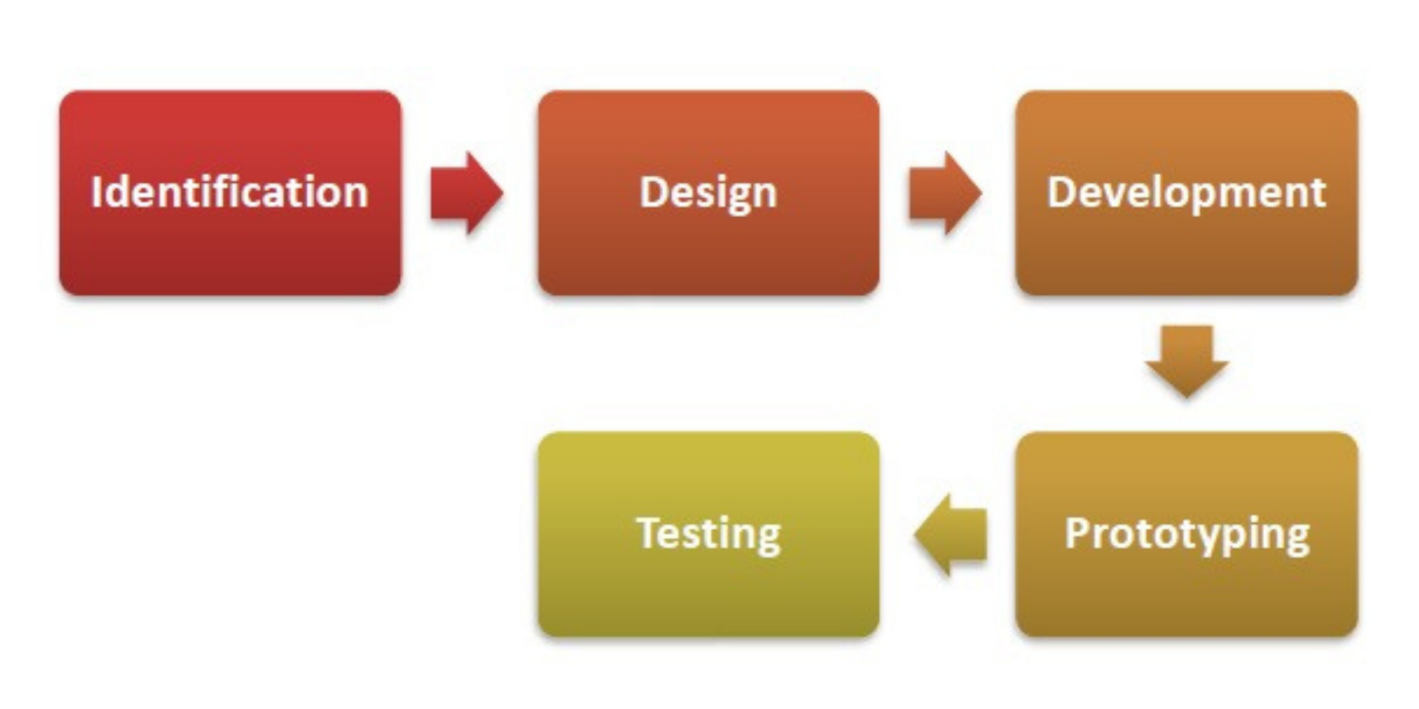
\includegraphics[width=0.8\linewidth]{mainmatter/images/madlc1.png}
    \caption{MADLC Phases Included in the Project}
    \caption*{Source: \textcite{moharekar21}}
    \caption*{\textit{Appropriated by: \textcite{shanmugam19}}}
    \label{fig:myfig32}
\end{figure}

The Mobile Application Development Life Cycle (MADLC) is a systematic approach introduced by \textcite{vithani14} to address various issues presented by mobile applications. These apps frequently include complex functionality that differs greatly from conventional desktop applications. The introduction of MADLC aimed to establish a structured framework for the development of mobile apps, recognizing the necessity for a customized approach \parencite{vithani14}. \\

\textcite{kaur15} addressed the significance of a dedicated development strategy for mobile applications, acknowledging their unique characteristics. \textcite{kaur15} also emphasize the necessity of adopting a unique methodology to address the unique characteristics and needs of mobile app development. MADLC addresses this requirement by providing a systematic and sequential approach that corresponds to the distinct difficulties and characteristics of mobile app development, including diverse screen sizes, device functionalities, and user expectations. \\

The Mobile Application Development Life Cycle (MADLC) consists of multiple stages that provide a structured framework for the development of mobile apps, as outlined by \textcite{wambua23} and explained by \textcite{wen21}. The following stages are crucial for developing mobile applications that achieve success:

\begin{enumerate}[1.]
    \item \textit{Identification:} The identification step involves identifying the problem statement and establishing the goal and objectives for creating the mobile application. System requirements are collected and the target audience is determined. Market research is performed to evaluate the potential viability of the application, and specific project scope and objectives are established.
    \item \textit{Design:} After the identification phase, the design phase begins. Developers are responsible for developing the user interface (UI) and user experience (UX) elements of the application. During this phase, flowcharts, Use Case Diagrams (UCD), Entity Relationship Diagrams (ERD), and Sequence Diagrams are generated. Wireframes, mockups, and prototypes are created to visually represent the structure and user experience. The selection of the suitable technology stack, databases, and architecture for the mobile application has been made.
    \item \textit{Development:} During the development phase, developers begin coding the mobile application, building its functionality according to the previously gathered design and specifications. This phase involves incorporating functionalities and ensuring consistency with the design and user experience principles. If necessary, backend systems, APIs, and server components are developed.
    \item \textit{Prototyping:} During this stage, the process of combining different systems and coding the front end and back end happens. Developers create a high-fidelity prototype of the mobile application, which includes important features and functions. The prototype plays a vital role in the development process by enabling the examination and verification of concepts and features. Early user feedback is sought and utilized to identify and address any design or functionality concerns before moving forward.
    \item \textit{Testing:} Quality assurance and testing are essential elements of MADLC. During this phase, a range of testing methods are employed, including functional testing, usability testing, performance testing, security testing, and compatibility testing across many devices and platforms. Testers detect and document defects and problems, which the developer then resolves to guarantee that the mobile application fulfills its functional specifications and provides a smooth user interface.
\end{enumerate}

These phases offer a systematic approach to the creation of mobile applications, guaranteeing that the outcome is in line with objectives, displays a strong design, undergoes comprehensive testing, and fulfills the requirements of its intended users. Nevertheless, it is critical to acknowledge that the MADLC has seven essential stages: identification, design, development, prototyping, testing, deployment, and maintenance. Within the scope of this project, the primary focus is on the early stages of the MADLC, specifically covering the identification to testing phases.
\pagebreak

\section{Methodology Development and Related Activities}
\subsection{Identification Phase}
\begin{table}[htb]
\caption{Overview of Identification Phase} 
\label{tab:mytable}
\centering
\begin{tabular}{|p{2.2cm}|p{2.6cm}|p{2.6cm}|p{2.6cm}|p{2.6cm}|}
\hline
\multicolumn{1}{|c|}{\textbf{Phase}} & 
\multicolumn{1}{c|}{\textbf{Objectives}} & 
\multicolumn{1}{c|}{\textbf{Activities}} & 
\multicolumn{1}{c|}{\textbf{Tools \& Techniques}} & 
\multicolumn{1}{c|}{\textbf{Deliverables}} \\
\hline 
\multirow{3}{*}{%
	\begin{tabular}[c]{@{}p{2.2cm}@{}}
	\vspace{4.4cm} \raggedright Identification \\[6pt]
	\end{tabular}
} &
\multirow{3}{*}{%
	\begin{tabular}[c]{@{}p{2.6cm}@{}}
	\vspace{1.8cm} \raggedright To identify system requirements for Alunan as a mobile application for local independent musicians' online community and music discovery \\[6pt]
	\end{tabular}
} &
\multirow{1}{*}{%
	\begin{tabular}[c]{@{}p{2.6cm}@{}}
	\vspace{0.6cm} \raggedright Collecting, gathering information and identifying the problem, objective, scope, and significance \\[6pt]
	\end{tabular}
} &
\raggedright Techniques: Literature Review \newline \newline Tools: Online Database UiTM, ResearchGate, IEEE Xplore, ScienceDirect, Scopus, \& Google Scholar &
\multirow{1}{*}{%
	\begin{tabular}[c]{@{}p{2.6cm}@{}}
	\vspace{0.5cm} \raggedright System requirements, Problem Statement, Objectives, Scope \& Significance \\[6pt]
	\end{tabular}
} \\ \cline{3-5}
& &
\multirow{1}{*}{%
	\begin{tabular}[c]{@{}p{2.6cm}@{}}
	\vspace{-0.1cm} \raggedright Define stakeholder characteristics \\[6pt]
	\end{tabular}
} &
\raggedright Technique: User Persona \newline \newline Tools: Canva & 
\multirow{1}{*}{%
	\begin{tabular}[c]{@{}p{2.6cm}@{}}
	\vspace{0.35cm} \raggedright User Persona \\[6pt]
	\end{tabular}
} \\ \cline{3-5}
& &
\multirow{1}{*}{%
	\begin{tabular}[c]{@{}p{2.6cm}@{}}
	\vspace{0.6cm} \raggedright Plan the timeline of the project \\[6pt]
	\end{tabular}
} &
\raggedright Techniques: Gantt Chart \newline \newline Tools: Lucidchart \& Canva & 
\multirow{1}{*}{%
	\begin{tabular}[c]{@{}p{2.6cm}@{}}
	\vspace{0.55cm} \raggedright Project Timeline (Gantt Chart) \\[6pt]
	\end{tabular}
} \\ \hline
\end{tabular}
\end{table}
Within the context of mobile application development, the identification phase, as described by \textcite{shanmugam19} and \textcite{wambua23}, includes the creation of new concepts and the execution of extensive research to determine the extent of application solutions, following the principles of computational thinking. Furthermore, \textcite{wambua23} highlights the need to gather ideas through brainstorming, improving existing concepts to increase originality, and doing initial requirements gathering to develop a strong foundation for the project. The identification step is crucial as it promotes the development of innovative solutions while also establishing a well-defined project scope and objectives.
\pagebreak

During this stage, key activities include gathering and collecting information to determine the problem, objectives, scope, and significance of the project. The process largely depends on performing an extensive literature review utilizing electronic resources such as Online Database UiTM, ResearchGate, IEEE Xplore, ScienceDirect, Scopus, and Google Scholar to acquire knowledge from previous research and solutions about the project's topic. The main outcomes of this phase include a well-defined problem statement, clear project objectives, and a properly defined scope and significance of the project. These deliverables serve as a guiding framework for the following stages of development, guaranteeing that the project stays in line with its objectives and effectively addresses the identified problem. \\

\begin{figure}[h]
    \centering
    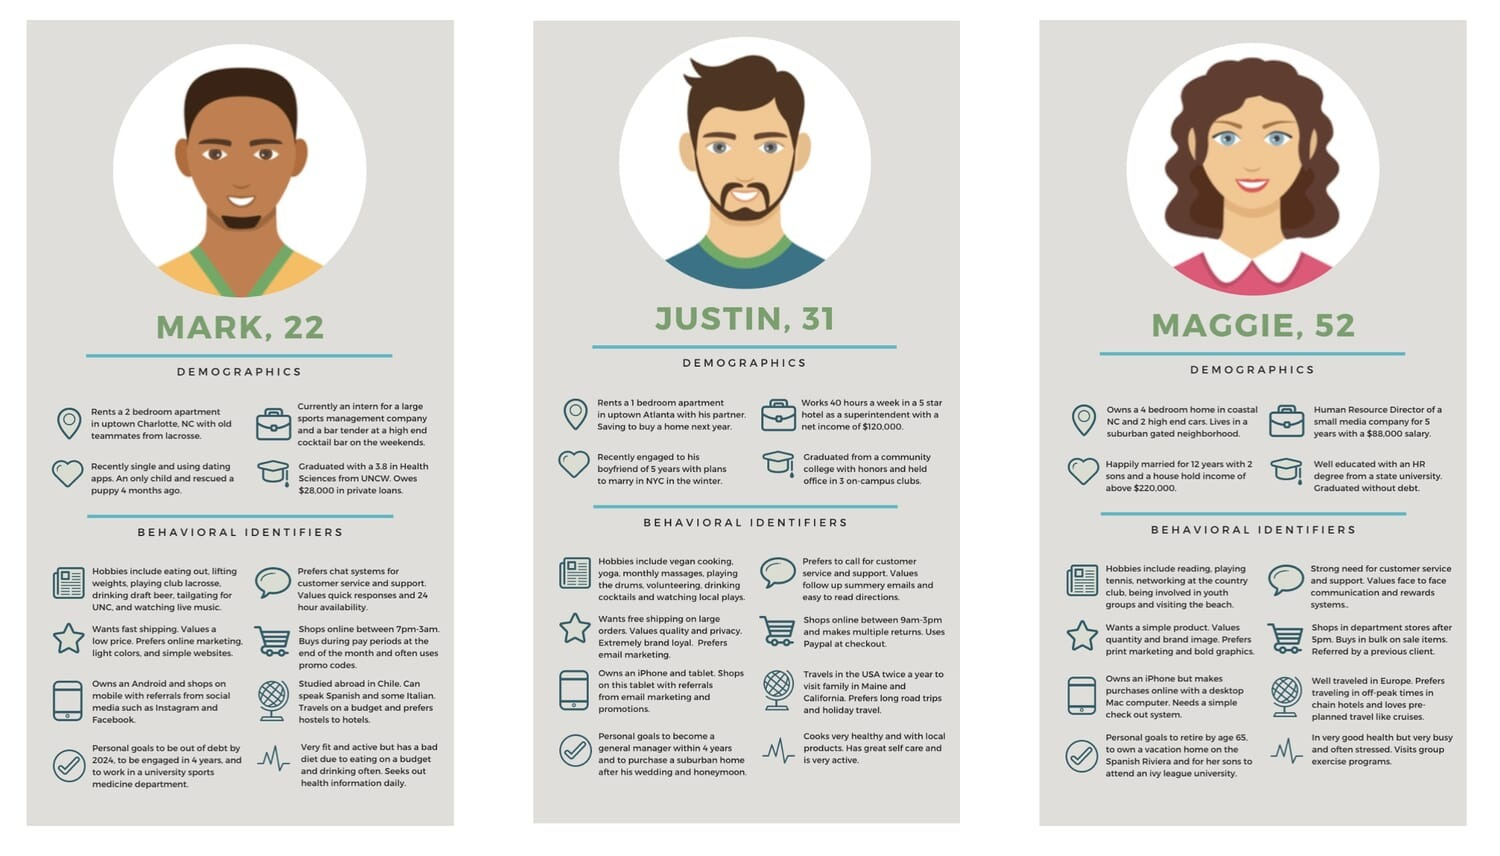
\includegraphics[width=0.8\linewidth]{mainmatter/images/exampleuserpersona.jpg}
	\caption{User Persona Example}
    \caption*{\textit{Personas: Are they the Answer for Visualizing Your User Research? [Boagworld, 2022]}}
    \caption*{https://boagworld.com/usability/personas/}
    \label{fig:myfig33}
\end{figure}

Furthermore, during the identification phase, stakeholder characteristics are determined by creating user personas, utilizing methods like user persona creation, and employing visual representation tools like Canva. Stakeholders are individuals or groups with a personal stake in the mobile application project, such as end-users and future clients. It is essential to understand the characteristics and needs of these stakeholders to customize the mobile application to properly fulfill their objectives.
\pagebreak

\begin{figure}[h]
    \centering
    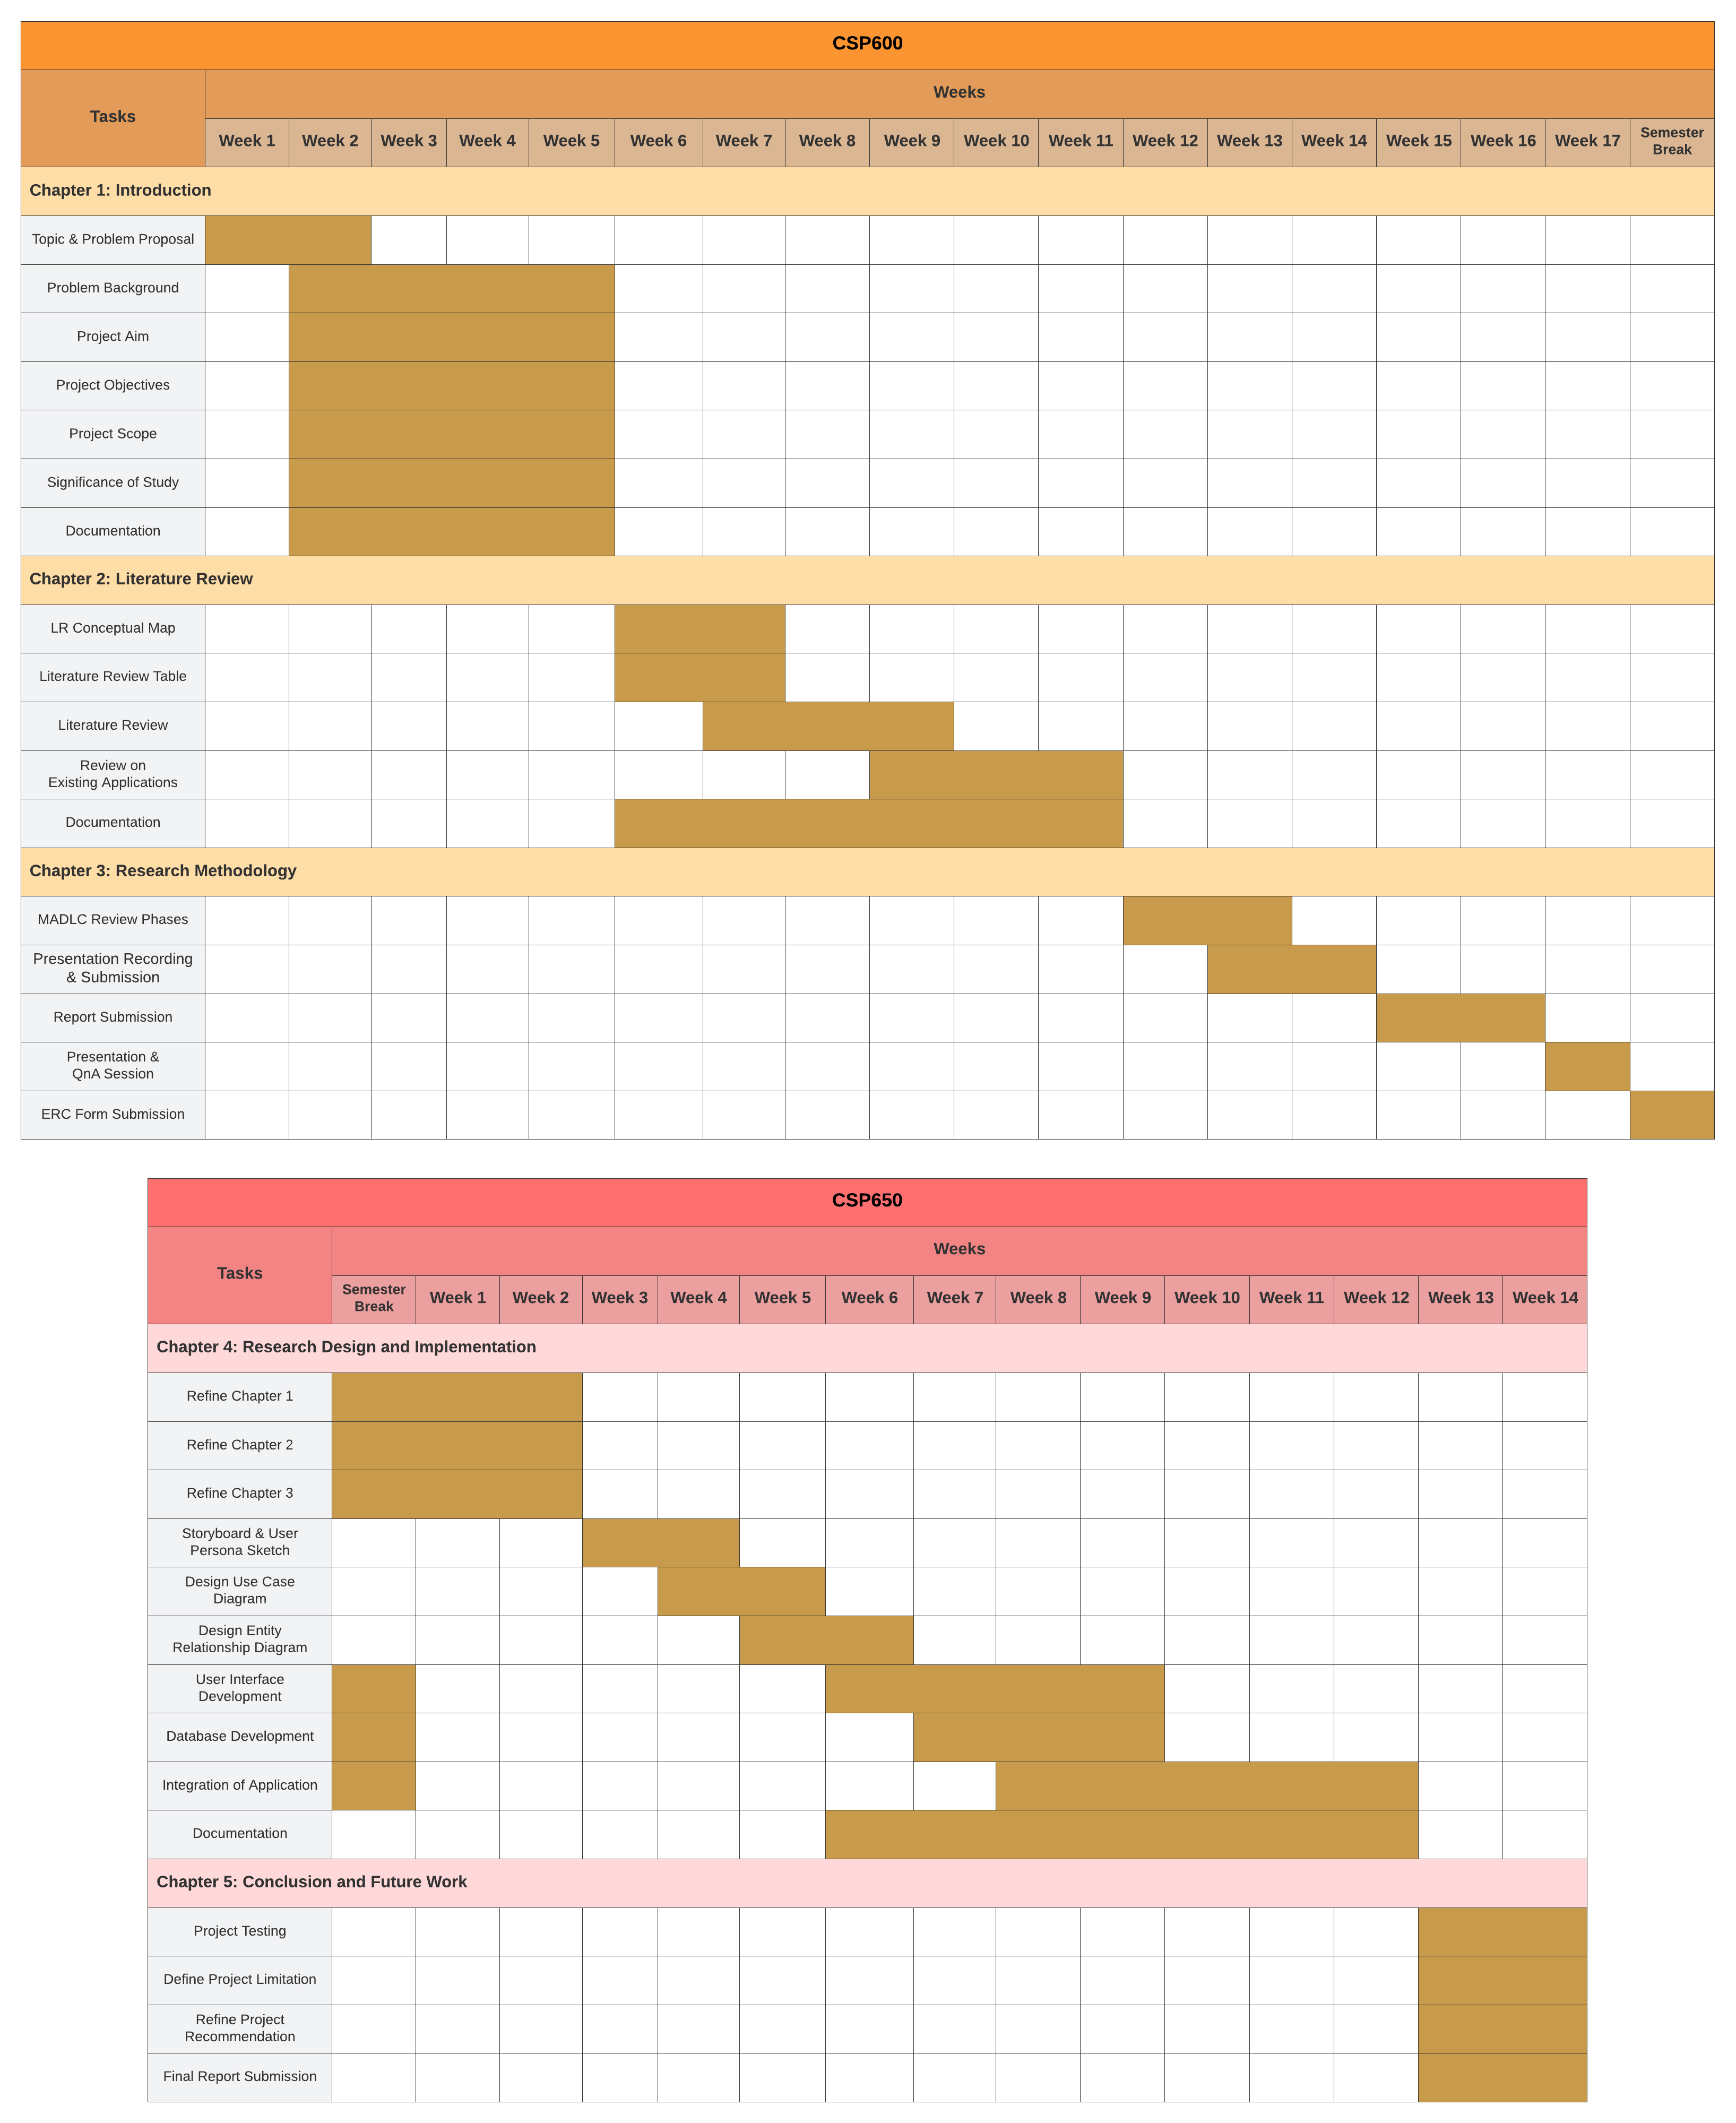
\includegraphics[width=0.8\linewidth]{mainmatter/images/ganttchart.png}
	\caption{Gantt Chart for Project Timeline}
    \label{fig:myfig34}
\end{figure}

In addition, project planning happens during this phase, which involves the development of a project timeline in the form of a Gantt Chart. The timetable for this project is created using online tools such as Lucidchart and Canva. These tools are used to visually represent the project's schedule, tasks, milestones, and dependencies. This enables effective control of the project's schedule, resources, and time limits, guaranteeing smooth progress through the development process.
\pagebreak

\subsection{Design Phase}
\begin{spacing}{1.0}
\begin{longtable}{|p{2.2cm}|p{2.6cm}|p{2.6cm}|p{2.6cm}|p{2.6cm}|}
\caption{Overview of Design Phase} 
\label{tab:mytable}\\
\hline
\multicolumn{1}{|c|}{\textbf{Phase}} & 
\multicolumn{1}{c|}{\textbf{Objectives}} & 
\multicolumn{1}{c|}{\textbf{Activities}} & 
\multicolumn{1}{c|}{\textbf{Tools \& Techniques}} & 
\multicolumn{1}{c|}{\textbf{Deliverables}} \\
\hline 
\endfirsthead % header for the first page
\multicolumn{5}{c}{{\tablename\ \thetable{} -- Continued from previous page}} \\
\hline
\multicolumn{1}{|c|}{\textbf{Phase}} & 
\multicolumn{1}{c|}{\textbf{Objectives}} & 
\multicolumn{1}{c|}{\textbf{Activities}} & 
\multicolumn{1}{c|}{\textbf{Tools \& Techniques}} & 
\multicolumn{1}{c|}{\textbf{Deliverables}} \\
\hline 
\endhead % header for subsequent pages
\multirow{7}{*}{%
	\begin{tabular}[c]{@{}p{2.2cm}@{}}
	\vspace{9.5cm} \raggedright Design \\[6pt]
	\end{tabular}
} &
\multirow{7}{*}{%
	\begin{tabular}[c]{@{}p{2.6cm}@{}}
	\vspace{7.5cm} \raggedright To design Alunan as a mobile application for local independent musicians’ online community and music discovery \\[6pt]
	\end{tabular}
} &
\multirow{1}{*}{%
	\begin{tabular}[c]{@{}p{2.6cm}@{}}
	\vspace{2cm} \raggedright Review existing apps and identify the hardware and software requirements \\[6pt]
	\end{tabular}
} &
\raggedright Techniques: Literature and research summary \newline \newline Tools: Google Play Store, Apple App Store, Microsoft Word, Laptop, Mobile Phone \& Google Chrome &
\multirow{1}{*}{%
	\begin{tabular}[c]{@{}p{2.6cm}@{}}
	\vspace{0.5cm} \raggedright Summary of design features and functions of existing applications \newline \newline Hardware and Software Requirements\\[6pt]
	\end{tabular}
} \\ \cline{3-5}
& &
\multirow{1}{*}{%
	\begin{tabular}[c]{@{}p{2.6cm}@{}}
	\vspace{1.15cm} \raggedright Outline system features \\[6pt]
	\end{tabular}
} &
\raggedright Technique: Requirement Analysis \newline \newline Tools: Google Chrome, Microsoft Word \& Canva & 
\multirow{1}{*}{%
	\begin{tabular}[c]{@{}p{2.6cm}@{}}
	\vspace{0.35cm} \raggedright Functional Requirements \& Non-Functional Requirements \\[6pt]
	\end{tabular}
} \\ \cline{3-5}
& &
\multirow{1}{*}{%
	\begin{tabular}[c]{@{}p{2.6cm}@{}}
	\vspace{0.8cm} \raggedright Designing User Interface \\[6pt]
	\end{tabular}
} &
\raggedright Techniques: Storyboard \& Wireframe \newline \newline Tools: Canva \& Figma & 
\multirow{1}{*}{%
	\begin{tabular}[c]{@{}p{2.6cm}@{}}
	\vspace{0.55cm} \raggedright Storyboard \& Wireframe \\[6pt]
	\end{tabular}
} \\ \cline{3-5}
& &
\multirow{4}{*}{%
	\begin{tabular}[c]{@{}p{2.6cm}@{}}
	\vspace{1.8cm} \raggedright Designing interaction flow for the app \\[6pt]
	\end{tabular}
} &
\raggedright Techniques: Flowchart \newline \newline Tools: Lucidchart \& Draw.io & 
\multirow{1}{*}{%
	\begin{tabular}[c]{@{}p{2.6cm}@{}}
	\vspace{0.55cm} \raggedright Flowcharts of the app \\[6pt]
	\end{tabular}
} \\ \cline{4-5}
& & &
\raggedright Techniques: Use Case Diagram (UCD) \newline \newline Tools: Lucidchart \& Draw.io & 
\multirow{1}{*}{%
	\begin{tabular}[c]{@{}p{2.6cm}@{}}
	\vspace{0.55cm} \raggedright Use Case Diagram (UCD) \\[6pt]
	\end{tabular}
} \\ \hline
& & &
\raggedright Techniques: Entity Relationship Diagram (ERD) \newline \newline Tools: Lucidchart \& Draw.io & 
\multirow{1}{*}{%
	\begin{tabular}[c]{@{}p{2.6cm}@{}}
	\vspace{0.55cm} \raggedright Entity Relationship Diagram (ERD) \\[6pt]
	\end{tabular}
} \\ \cline{4-5}
& & &
\raggedright Techniques: Sequence Diagram \newline \newline Tools: Lucidchart \& Draw.io & 
\multirow{1}{*}{%
	\begin{tabular}[c]{@{}p{2.6cm}@{}}
	\vspace{0.55cm} \raggedright Sequence Diagram \\[6pt]
	\end{tabular}
} \\ \hline
\end{longtable}
\end{spacing}

In the Mobile Application Development Lifecycle (MADLC), the design phase is a crucial stage where the initial ideas and plans for the project are transformed into an actual form. In this stage, a detailed plan is developed which includes all the necessary design elements, hardware and software needs, and architectural frameworks for the mobile application. This plan is created to ensure that it aligns with the project's goals and objectives. According to \textcite{wambua23}, the first step in the design process involves determining the functional needs and making important decisions. According to \textcite{shanmugam19}, it is recommended for developers to construct a storyboard outlining the flow of the user interface design for the application. This step is crucial for visually illustrating the design of the program, enabling a thorough description of its flow and interactions. \\

In the project's context, the design phase begins by conducting an in-depth review of mobile applications that are relevant to the project's domain. This involves reviewing applications from popular app stores like Google Play Store and Apple Store, as well as undertaking thorough research to determine the precise hardware and software requirements that align with the project's objectives. The tools utilized for this project include a laptop, smartphone, Google Chrome, and Microsoft Word. The main outputs consist of a concise review of design characteristics and functionalities derived from current applications, together with a thorough inventory of hardware and software requirements customized to meet the project's specific requirements. \\

\begin{table}[htb]
\caption{Hardware Requirements} 
\label{tab:mytable}
\centering
\begin{tabular}{|p{0.5cm}|p{3cm}|p{3cm}|p{6cm}|}
\hline
\multicolumn{1}{|c|}{\textbf{No}} & 
\multicolumn{1}{c|}{\textbf{Hardware}} & 
\multicolumn{2}{c|}{\textbf{Specification}} \\
\hline
\multirow{4}{*}{%
	\begin{tabular}[c]{@{}p{0.5cm}@{}}
	\vspace{-0.05cm} \raggedright 1 \\
	\end{tabular}
} &
\multirow{4}{*}{%
	\begin{tabular}[c]{@{}p{3cm}@{}}
	\vspace{-0.05cm} \raggedright PC or Laptop \\
	\end{tabular}
} &
\multirow{1}{*}{%
	\begin{tabular}[c]{@{}p{3cm}@{}}
	\raggedright Processor \\
	\end{tabular}
} &
\multirow{1}{*}{%
	\begin{tabular}[c]{@{}p{6cm}@{}}
	\raggedright Intel Core i5 or AMD Ryzen 5 \\
	\end{tabular}
} \\ \cline{3-4}
& &
\multirow{1}{*}{%
	\begin{tabular}[c]{@{}p{3cm}@{}}
	\raggedright RAM \\
	\end{tabular}
} &
\multirow{1}{*}{%
	\begin{tabular}[c]{@{}p{6cm}@{}}
	\raggedright 8GB or higher \\
	\end{tabular}
} \\ \cline{3-4}
& &
\multirow{1}{*}{%
	\begin{tabular}[c]{@{}p{3cm}@{}}
	\raggedright Storage \\
	\end{tabular}
} &
\multirow{1}{*}{%
	\begin{tabular}[c]{@{}p{6cm}@{}}
	\raggedright 256GB SSD or HDD \\
	\end{tabular}
} \\ \cline{3-4}
& &
\multirow{1}{*}{%
	\begin{tabular}[c]{@{}p{3cm}@{}}
	\raggedright Operating System \\
	\end{tabular}
} &
\multirow{1}{*}{%
	\begin{tabular}[c]{@{}p{6cm}@{}}
	\raggedright Windows 10 or higher \\
	\end{tabular}
} \\ \hline
& & & \\
\multirow{4}{*}{%
	\begin{tabular}[c]{@{}p{0.5cm}@{}}
	\raggedright 2 \\
	\end{tabular}
} &
\multirow{4}{*}{%
	\begin{tabular}[c]{@{}p{3cm}@{}}
	\raggedright Mobile Phone or Tablet \\
	\end{tabular}
} &
\multirow{1}{*}{%
	\begin{tabular}[c]{@{}p{3cm}@{}}
	\vspace{-0.55cm} \raggedright Model \\
	\end{tabular}
} &
\multirow{1}{*}{%
	\begin{tabular}[c]{@{}p{6cm}@{}}
	\vspace{-0.8cm} \raggedright Any modern smartphone or tablet with decent performance \\[6pt]
	\end{tabular}
} \\ \cline{3-4}
& &
\multirow{1}{*}{%
	\begin{tabular}[c]{@{}p{3cm}@{}}
	\raggedright CPU \\
	\end{tabular}
} &
\multirow{1}{*}{%
	\begin{tabular}[c]{@{}p{6cm}@{}}
	\raggedright Qualcomm Snapdragon 660 or higher \\
	\end{tabular}
} \\ \cline{3-4}
& &
\multirow{1}{*}{%
	\begin{tabular}[c]{@{}p{3cm}@{}}
	\raggedright RAM \\
	\end{tabular}
} &
\multirow{1}{*}{%
	\begin{tabular}[c]{@{}p{6cm}@{}}
	\raggedright 4GB or higher \\
	\end{tabular}
} \\ \cline{3-4}
& &
\multirow{1}{*}{%
	\begin{tabular}[c]{@{}p{3cm}@{}}
	\raggedright Storage \\
	\end{tabular}
} &
\multirow{1}{*}{%
	\begin{tabular}[c]{@{}p{6cm}@{}}
	\raggedright Minimum 64GB internal storage \\
	\end{tabular}
} \\ \hline
\end{tabular}
\end{table}

\begin{table}[htb]
\caption{Software Requirements} 
\label{tab:mytable}
\centering
\begin{tabular}{|p{0.5cm}|p{3.5cm}|p{9cm}|}
\hline
\multicolumn{1}{|c|}{\textbf{No}} & 
\multicolumn{1}{c|}{\textbf{Software}} & 
\multicolumn{1}{c|}{\textbf{Descriptions}} \\
\hline
\multirow{1}{*}{%
	\begin{tabular}[c]{@{}p{0.5cm}@{}}
	\raggedright 1 \\
	\end{tabular}
} &
\multirow{1}{*}{%
	\begin{tabular}[c]{@{}p{2.5cm}@{}}
	\raggedright Figma \\
	\end{tabular}
} &
\multirow{1}{*}{%
	\begin{tabular}[c]{@{}p{10cm}@{}}
	\raggedright To create the user interface for the application \\
	\end{tabular}
} \\ \hline
\multirow{1}{*}{%
	\begin{tabular}[c]{@{}p{0.5cm}@{}}
	\raggedright 2 \\
	\end{tabular}
} &
\multirow{1}{*}{%
	\begin{tabular}[c]{@{}p{2.5cm}@{}}
	\raggedright Canva \\
	\end{tabular}
} &
\multirow{1}{*}{%
	\begin{tabular}[c]{@{}p{10cm}@{}}
	\raggedright To create user persona for this project \\
	\end{tabular}
} \\ \hline
\multirow{1}{*}{%
	\begin{tabular}[c]{@{}p{0.5cm}@{}}
	\raggedright 3 \\
	\end{tabular}
} &
\multirow{1}{*}{%
	\begin{tabular}[c]{@{}p{2.5cm}@{}}
	\raggedright Lucidchart \\
	\end{tabular}
} &
\multirow{1}{*}{%
	\begin{tabular}[c]{@{}p{10cm}@{}}
	\raggedright To create a Gantt chart for the project \\
	\end{tabular}
} \\ \hline
\multirow{1}{*}{%
	\begin{tabular}[c]{@{}p{0.5cm}@{}}
	\raggedright 4 \\
	\end{tabular}
} &
\multirow{1}{*}{%
	\begin{tabular}[c]{@{}p{2.5cm}@{}}
	\raggedright Draw.io \\
	\end{tabular}
} &
\multirow{1}{*}{%
	\begin{tabular}[c]{@{}p{10cm}@{}}
	\raggedright To create the interaction flow for the application  \\
	\end{tabular}
} \\ \hline
\multirow{1}{*}{%
	\begin{tabular}[c]{@{}p{0.5cm}@{}}
	\raggedright 5 \\
	\end{tabular}
} &
\multirow{1}{*}{%
	\begin{tabular}[c]{@{}p{4cm}@{}}
	\raggedright Google Play Store \\
	\end{tabular}
} &
\multirow{1}{*}{%
	\begin{tabular}[c]{@{}p{10cm}@{}}
	\raggedright To compare similar applications \\
	\end{tabular}
} \\ \hline
\multirow{1}{*}{%
	\begin{tabular}[c]{@{}p{0.5cm}@{}}
	\raggedright 6 \\
	\end{tabular}
} &
\multirow{1}{*}{%
	\begin{tabular}[c]{@{}p{4cm}@{}}
	\raggedright Apple App Store \\
	\end{tabular}
} &
\multirow{1}{*}{%
	\begin{tabular}[c]{@{}p{10cm}@{}}
	\raggedright To compare similar applications \\
	\end{tabular}
} \\ \hline
\multirow{1}{*}{%
	\begin{tabular}[c]{@{}p{0.5cm}@{}}
	\raggedright 7 \\
	\end{tabular}
} &
\multirow{1}{*}{%
	\begin{tabular}[c]{@{}p{2.5cm}@{}}
	\raggedright Microsoft Word \\
	\end{tabular}
} &
\multirow{1}{*}{%
	\begin{tabular}[c]{@{}p{10cm}@{}}
	\raggedright To create the documentation and reports of the project \\
	\end{tabular}
} \\ \hline
\multirow{1}{*}{%
	\begin{tabular}[c]{@{}p{0.5cm}@{}}
	\raggedright 8 \\
	\end{tabular}
} &
\multirow{1}{*}{%
	\begin{tabular}[c]{@{}p{4cm}@{}}
	\raggedright Visual Studio Code \\
	\end{tabular}
} &
\multirow{1}{*}{%
	\begin{tabular}[c]{@{}p{10cm}@{}}
	\raggedright To create the documentation and reports of the project \\
	\end{tabular}
} \\ \hline
\multirow{1}{*}{%
	\begin{tabular}[c]{@{}p{0.5cm}@{}}
	\raggedright 9 \\
	\end{tabular}
} &
\multirow{1}{*}{%
	\begin{tabular}[c]{@{}p{2.5cm}@{}}
	\raggedright Google Chrome \\
	\end{tabular}
} &
\multirow{1}{*}{%
	\begin{tabular}[c]{@{}p{10cm}@{}}
	\raggedright To browse the journal, articles, and books \\
	\end{tabular}
} \\ \hline
\multirow{1}{*}{%
	\begin{tabular}[c]{@{}p{0.5cm}@{}}
	\raggedright 10 \\
	\end{tabular}
} &
\multirow{1}{*}{%
	\begin{tabular}[c]{@{}p{2.5cm}@{}}
	\raggedright Android Studio \\
	\end{tabular}
} &
\multirow{1}{*}{%
	\begin{tabular}[c]{@{}p{10cm}@{}}
	\raggedright To develop the front-end and back-end of the application \\
	\end{tabular}
} \\ \hline
\multirow{1}{*}{%
	\begin{tabular}[c]{@{}p{0.5cm}@{}}
	\raggedright 11 \\
	\end{tabular}
} &
\multirow{1}{*}{%
	\begin{tabular}[c]{@{}p{2.5cm}@{}}
	\raggedright Firebase \\
	\end{tabular}
} &
\multirow{1}{*}{%
	\begin{tabular}[c]{@{}p{10cm}@{}}
	\raggedright To develop a database of the application \\
	\end{tabular}
} \\ \hline
\multirow{1}{*}{%
	\begin{tabular}[c]{@{}p{0.5cm}@{}}
	\raggedright 12 \\
	\end{tabular}
} &
\multirow{1}{*}{%
	\begin{tabular}[c]{@{}p{2.5cm}@{}}
	\raggedright Google Forms \\
	\end{tabular}
} &
\multirow{1}{*}{%
	\begin{tabular}[c]{@{}p{10cm}@{}}
	\raggedright To create SUS Questionnaire for user testing \\
	\end{tabular}
} \\ \hline
\multirow{1}{*}{%
	\begin{tabular}[c]{@{}p{0.5cm}@{}}
	\raggedright 13 \\
	\end{tabular}
} &
\multirow{1}{*}{%
	\begin{tabular}[c]{@{}p{4cm}@{}}
	\raggedright Google Spreadsheet \\
	\end{tabular}
} &
\multirow{1}{*}{%
	\begin{tabular}[c]{@{}p{10cm}@{}}
	\raggedright To calculate SUS score based on user testing \\
	\end{tabular}
} \\ \hline
\multirow{1}{*}{%
	\begin{tabular}[c]{@{}p{0.5cm}@{}}
	\raggedright 14 \\
	\end{tabular}
} &
\multirow{1}{*}{%
	\begin{tabular}[c]{@{}p{2.5cm}@{}}
	\raggedright GitHub \\
	\end{tabular}
} &
\multirow{1}{*}{%
	\begin{tabular}[c]{@{}p{10cm}@{}}
	\raggedright To control version of the application and report \\
	\end{tabular}
} \\ \hline
\end{tabular}
\end{table}

Within the project's framework, the design phase entails the thorough identification of system features. This is accomplished through an in-depth requirement analysis process, in which both functional and non-functional requirements are discovered and carefully documented. The documentation process is facilitated by employing techniques like requirement analysis and utilizing applications like Google Chrome, Microsoft Word, and Canva. The primary deliverables consist of functional requirements that identify the functionality of the application, and also non-functional requirements that define characteristics such as performance, security, and others. \\

As part of the project, the design phase progresses by developing the user interface (UI) of the program. This task requires using methods such as storyboarding and wireframing to visually represent and strategize user interface components. Canva and Figma are digital tools used for design purposes. The main deliverables consist of storyboard and wireframe representations, which visually outline the interface of the program and ensure that it aligns with the user experience objectives. \\

\begin{figure}[ht]
    \centering
	\begin{tabular}{|c|c|}
		\hline
		\begin{subfigure}[b]{0.44\textwidth}
			\centering
			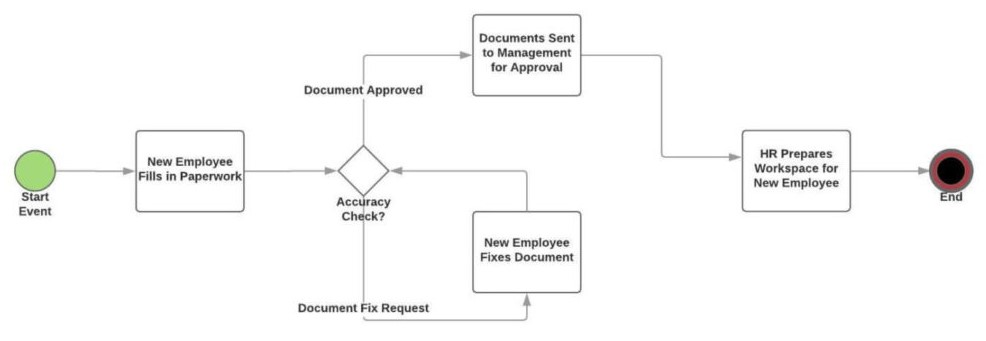
\includegraphics[width=0.9\linewidth]{mainmatter/images/exampleflowchart.jpeg}
			\caption{Flowchart}
         	\label{fig:myfig35}
		\end{subfigure} & 
		\begin{subfigure}[b]{0.44\textwidth}
			\centering
			\vspace{0.2cm}
			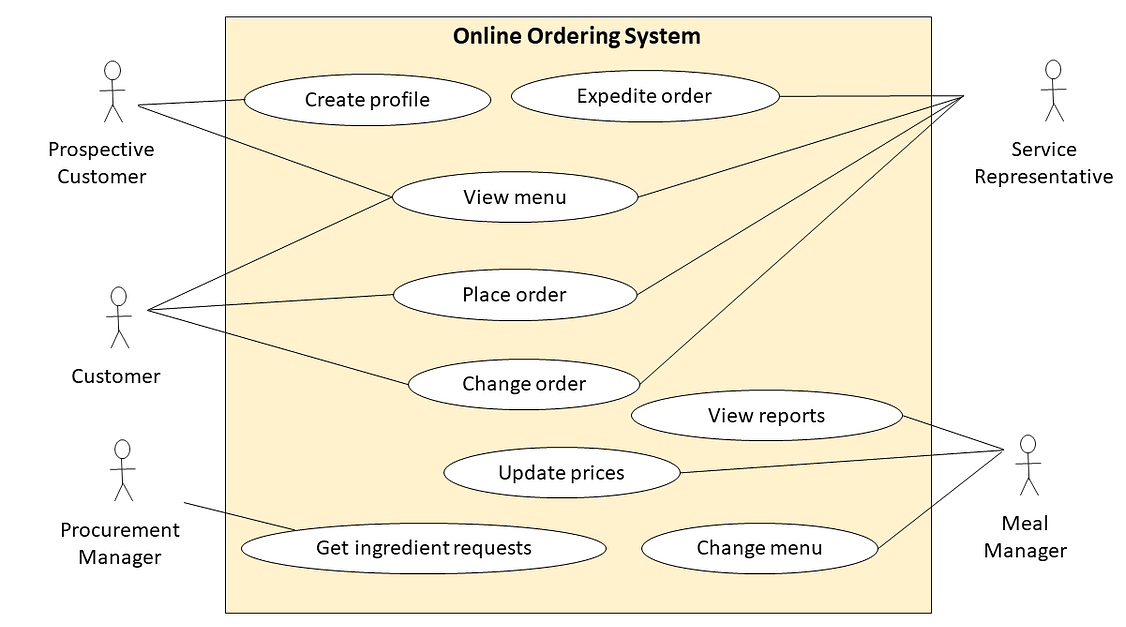
\includegraphics[width=0.7\linewidth]{mainmatter/images/exampleucd.png}
			\caption{User Case Diagram (UCD)}
         	\label{fig:myfig36}
		\end{subfigure}	\\
		\hline
		\begin{subfigure}[b]{0.44\textwidth}
			\centering
			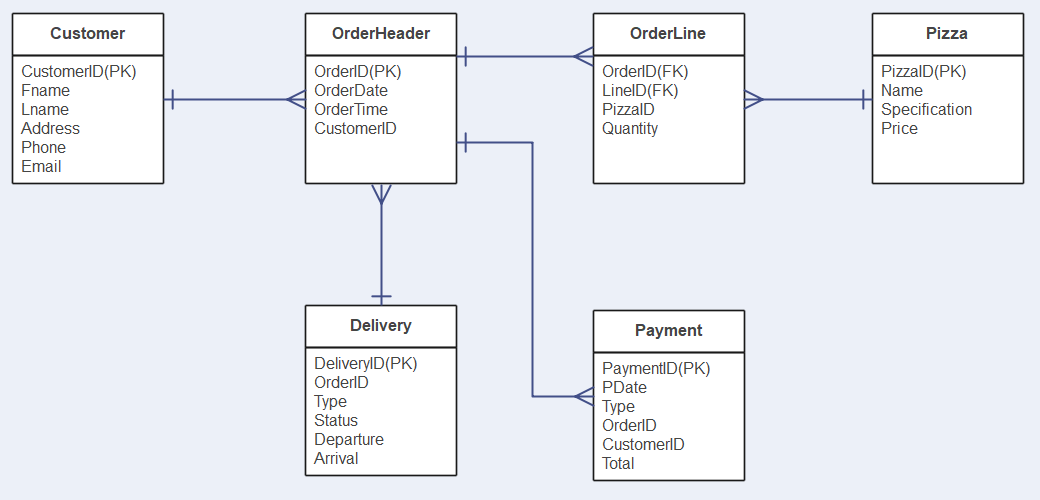
\includegraphics[width=0.8\linewidth]{mainmatter/images/exampleerd.png}
			\caption{Entity Relationship Diagram (ERD)}
         	\label{fig:myfig37}
		\end{subfigure} & 
		\begin{subfigure}[b]{0.44\textwidth}
			\centering
			\vspace{0.2cm}
			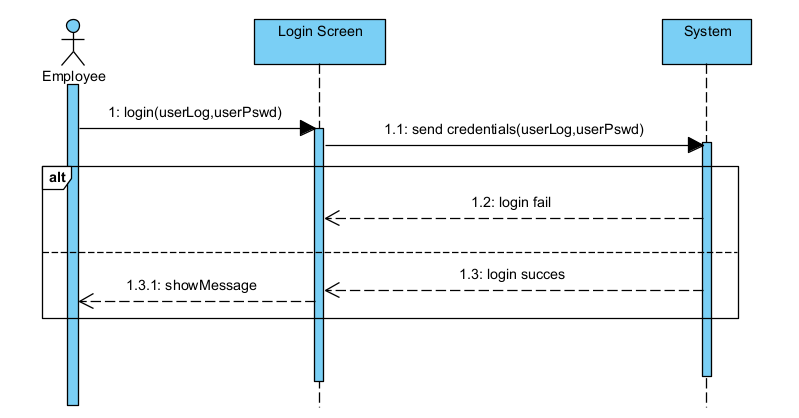
\includegraphics[width=0.8\linewidth]{mainmatter/images/examplesequencediagram.png}
			\caption{Sequence Diagram}
         	\label{fig:myfig38}
		\end{subfigure}	\\
		\hline		
	\end{tabular}
    \caption{Design Phase Deliverables Examples}
	\caption*{\textit{[SmartDraw, 2023], [Medium, 2022], [EDraw, 2022] \& [Stack Overflow, 2022]}}
    \label{fig:the4fig}
\end{figure}

As the project progresses, the design phase now focuses on creating the interaction flow for the mobile application. This entails utilizing methodologies such as creating flowcharts and employing Use Case Diagrams (UCD), Entity Relationship Diagrams (ERD), and Sequence Diagrams to illustrate the functionalities and interactions of the application. Lucidchart and Draw.io, are used to assist in the production of these diagrams. The main outputs comprise flowcharts, Use Case Diagrams (UCDs), Entity-Relationship Diagrams (ERDs), and Sequence Diagrams. These outputs offer a full representation of the user's interaction with the application and the flow of data within the system.
\pagebreak

\subsection{Development Phase}
\begin{table}[htb]
\caption{Overview of Development Phase} 
\label{tab:mytable}
\centering
\begin{tabular}{|p{2.2cm}|p{2.6cm}|p{2.6cm}|p{2.6cm}|p{2.6cm}|}
\hline
\multicolumn{1}{|c|}{\textbf{Phase}} & 
\multicolumn{1}{c|}{\textbf{Objectives}} & 
\multicolumn{1}{c|}{\textbf{Activities}} & 
\multicolumn{1}{c|}{\textbf{Tools \& Techniques}} & 
\multicolumn{1}{c|}{\textbf{Deliverables}} \\
\hline 
\multirow{2}{*}{%
	\begin{tabular}[c]{@{}p{2.2cm}@{}}
	\vspace{2.3cm} \raggedright Development \\[6pt]
	\end{tabular}
} &
\multirow{2}{*}{%
	\begin{tabular}[c]{@{}p{2.6cm}@{}}
	\vspace{0.4cm} \raggedright To develop the Alunan as a mobile application for local independent musicians’ online community and music discovery \\[6pt]
	\end{tabular}
} &
\multirow{1}{*}{%
	\begin{tabular}[c]{@{}p{2.6cm}@{}}
	\vspace{0.45cm} \raggedright Develop user interface and functionalities \\[6pt]
	\end{tabular}
} &
\raggedright Techniques: User Interface Development \newline \newline Tools: Android Studio \& Figma &
\multirow{1}{*}{%
	\begin{tabular}[c]{@{}p{2.6cm}@{}}
	\vspace{-0.07cm} \raggedright User Interface for Alunan mobile application developed \\[6pt]
	\end{tabular}
} \\ \cline{3-5}
& &
\multirow{1}{*}{%
	\begin{tabular}[c]{@{}p{2.6cm}@{}}
	\vspace{0.35cm} \raggedright Establish database for the mobile application \\[6pt]
	\end{tabular}
} &
\raggedright Technique: Database Development \newline \newline Tools: Android Studio \& Firebase & 
\multirow{1}{*}{%
	\begin{tabular}[c]{@{}p{2.6cm}@{}}
	\vspace{0.38cm} \raggedright Database for Alunan mobile application created \\[6pt]
	\end{tabular}
} \\ \hline
\end{tabular}
\end{table}

The development phase in the Mobile Application Development Lifecycle (MADLC) is a crucial step where the project's conceptualization and design are transformed into concrete implementation. In this stage, the interface design, as described by \textcite{shanmugam19}, is combined with the selected programming language. The development process is essentially divided into two distinct components: functional programming, which deals with the application's scope and goal, and programming for the user interface, which includes multimedia elements such as buttons, hyperlinks, and images. According to \textcite{wambua23}, a suitable programming language is deliberately selected to write the code for the mobile application's functional needs and user interface. This programming language acts as the underlying framework for the application's functionality and user interactions, ensuring that the design specifications are accurately converted into executable code. \\

The development phase involves the initial set of tasks, mostly focused on creating the user interface along with crucial features. The development of the user interface is carried out carefully, employing tools like Android Studio and Figma to design a user-friendly and feature-packed interface that is customized to meet the specific requirements of the application. The main outcome resulting from these efforts is a well-designed user interface that smoothly aligns with the aims of the application. \\

\begin{figure}[h]
    \centering
    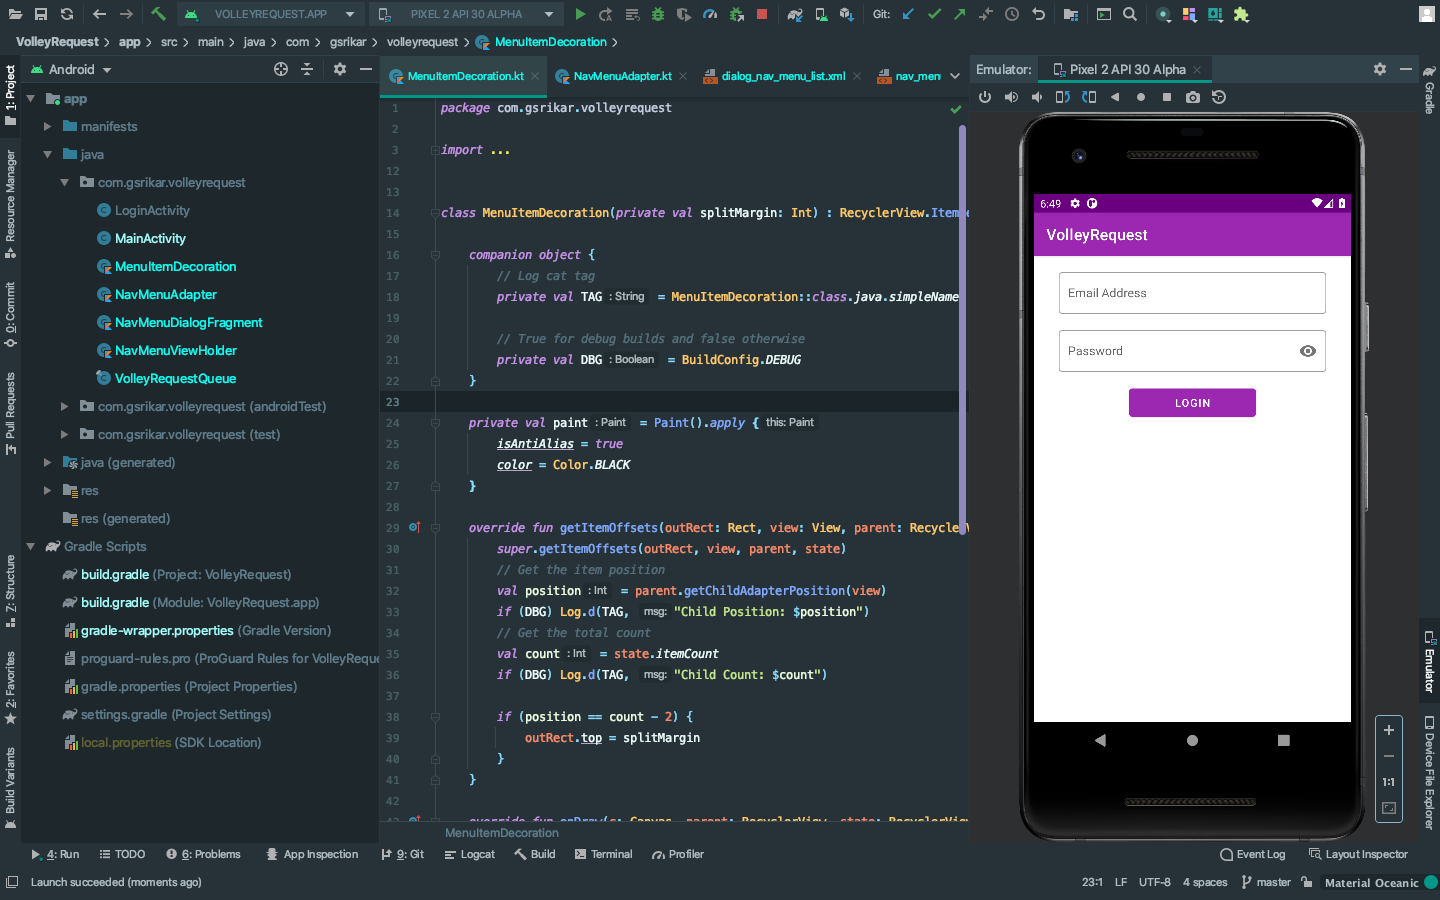
\includegraphics[width=0.9\linewidth]{mainmatter/images/ssandroidstudio.png}
	\caption{Screenshot of Android Studio}
    \caption*{\textit{Android Studio: Emulators [Cloud2Data, 2023]}}
    \caption*{https://cloud2data.com/android-studio-emulators/}
    \label{fig:myfig39}
\end{figure}

Alongside the construction of the user interface, the development phase also includes the creation of a strong and organized database. This activity entails the utilization of database development techniques, frequently utilizing Android Studio and Firebase as essential tools. The primary objective is to establish a database that can effectively store and retrieve data, serving as a fundamental element essential for the smooth functioning of the mobile application. These development activities serve as the connection between the project's design and its actual implementation, laying the foundation for the future testing stage in the mobile application development process.
\pagebreak

\subsection{Prototyping Phase}
\begin{table}[htb]
\caption{Overview of Prototyping Phase} 
\label{tab:mytable}
\centering
\begin{tabular}{|p{2.2cm}|p{2.6cm}|p{2.6cm}|p{2.6cm}|p{2.6cm}|}
\hline
\multicolumn{1}{|c|}{\textbf{Phase}} & 
\multicolumn{1}{c|}{\textbf{Objectives}} & 
\multicolumn{1}{c|}{\textbf{Activities}} & 
\multicolumn{1}{c|}{\textbf{Tools \& Techniques}} & 
\multicolumn{1}{c|}{\textbf{Deliverables}} \\
\hline 
\multirow{2}{*}{%
	\begin{tabular}[c]{@{}p{2.2cm}@{}}
	\vspace{3.4cm} \raggedright Prototyping \\[6pt]
	\end{tabular}
} &
\multirow{2}{*}{%
	\begin{tabular}[c]{@{}p{2.6cm}@{}}
	\vspace{1.4cm} \raggedright To develop the Alunan as a mobile application for local independent musicians’ online community and music discovery \\[6pt]
	\end{tabular}
} &
\multirow{1}{*}{%
	\begin{tabular}[c]{@{}p{2.6cm}@{}}
	\vspace{1.05cm} \raggedright System Integration and Frontend-Backend Coding \\[6pt]
	\end{tabular}
} &
\raggedright Techniques: Frontend and Backend coding and System Integration Coding \newline \newline Tools: Android Studio \& Firebase &
\multirow{1}{*}{%
	\begin{tabular}[c]{@{}p{2.6cm}@{}}
	\vspace{0.75cm} \raggedright Coding algorithms that integrate the frontend and backend elements \\[6pt]
	\end{tabular}
} \\ \cline{3-5}
& &
\multirow{1}{*}{%
	\begin{tabular}[c]{@{}p{2.6cm}@{}}
	\vspace{0.2cm} \raggedright Construct a high-fidelity Alunan app prototype with key features and interactions \\[6pt]
	\end{tabular}
} &
\raggedright Technique: High-Fidelity Prototyping \newline \newline Tools: \newline Android Studio, \newline Firebase \& \newline Tablet & 
\multirow{1}{*}{%
	\begin{tabular}[c]{@{}p{2.6cm}@{}}
	\vspace{-0.1cm} \raggedright A high-fidelity prototype of the Alunan mobile application that includes key features and interactions \\[6pt]
	\end{tabular}
} \\ \hline
\end{tabular}
\end{table}

The prototyping phase in the Mobile Application Development Lifecycle (MADLC) is defined by its focus on producing realistic representations of the Alunan mobile application's user interface (UI) and functionality. In this stage, the main goal is to create prototypes or mockups that provide stakeholders with a visual and interactive preview of the application's design and functionalities. This helps them better comprehend how the application will look and work. According to \textcite{shanmugam19} and \textcite{wambua23}, this phase is critical since it is necessary to ensure that the application is in line with the established standards. \\

Within the context of the Alunan mobile application project, the prototyping phase consists of a variety of crucial actions. First and foremost, system integration and frontend-backend coding are of primary importance. This requires the careful execution of frontend and backend code pieces, with a focus on integrating these components to guarantee smooth functionality. The activities commonly involve the use of Android Studio and Firebase, which are crucial for developing codes that allow the integration of frontend and backend components. The deliverables of this phase include coding methods that enable the smooth integration of frontend and backend components, establishing the foundation for the following development stages. \\

In addition, as part of the Alunan mobile application project, the prototyping phase involves creating a high-fidelity prototype. This significant effort involves developing a realistic and interactive depiction of the Alunan application, including its essential features and functions. High-fidelity prototyping techniques are utilized to ensure that the prototype accurately reflects the intended final product. By utilizing tools such as Android Studio and Firebase with a tablet device, the goal is to create a high-fidelity prototype that accurately represents the key features and interactions of the Alunan mobile application. The outcome of this process is a high-fidelity prototype that acts as a detailed and accurate representation, providing stakeholders with a tangible preview of the application's essential features and user experience.
\pagebreak

\subsection{Testing Phase}
\begin{table}[htb]
\caption{Overview of Testing Phase} 
\label{tab:mytable}
\centering
\begin{tabular}{|p{2.2cm}|p{2.6cm}|p{2.6cm}|p{2.6cm}|p{2.6cm}|}
\hline
\multicolumn{1}{|c|}{\textbf{Phase}} & 
\multicolumn{1}{c|}{\textbf{Objectives}} & 
\multicolumn{1}{c|}{\textbf{Activities}} & 
\multicolumn{1}{c|}{\textbf{Tools \& Techniques}} & 
\multicolumn{1}{c|}{\textbf{Deliverables}} \\
\hline 
\multirow{2}{*}{%
	\begin{tabular}[c]{@{}p{2.2cm}@{}}
	\vspace{3.4cm} \raggedright Testing \\[6pt]
	\end{tabular}
} &
\multirow{2}{*}{%
	\begin{tabular}[c]{@{}p{2.6cm}@{}}
	\vspace{1.4cm} \raggedright To develop the Alunan as a mobile application for local independent musicians’ online community and music discovery \\[6pt]
	\end{tabular}
} &
\multirow{1}{*}{%
	\begin{tabular}[c]{@{}p{2.6cm}@{}}
	\vspace{0.65cm} \raggedright Perform application testing \\[6pt]
	\end{tabular}
} &
\raggedright Techniques: Android Emulator \newline \newline Tools: Android Studio, Firebase \& Tablet &
\multirow{1}{*}{%
	\begin{tabular}[c]{@{}p{2.6cm}@{}}
	\vspace{0.78cm} \raggedright Result of Testing \\[6pt]
	\end{tabular}
} \\ \cline{3-5}
& &
\multirow{1}{*}{%
	\begin{tabular}[c]{@{}p{2.6cm}@{}}
	\vspace{1cm} \raggedright Perform usability and user acceptance testing \\[6pt]
	\end{tabular}
} &
\raggedright Technique: System Usability Scale (SUS) Questionnaire \newline \newline Tools: \newline Google Form \& \newline Google Spreadsheet & 
\multirow{1}{*}{%
	\begin{tabular}[c]{@{}p{2.6cm}@{}}
	\vspace{1.45cm} \raggedright SUS Score and User Feedback \\[6pt]
	\end{tabular}
} \\ \hline
\end{tabular}
\end{table}

The testing phase in the Mobile Application Development Lifecycle (MADLC) is extremely important, especially because it involves targeted users and real devices for thorough testing. At this step, an in-depth evaluation and testing of the mobile application are carried out to guarantee that its performance and functionality meet the required standards \parencite{shanmugam19}. During this testing phase, the application's reliability and adaptability for real-world usage scenarios are comprehensively assessed and improved. In addition, as stated by \textcite{wambua23}, the testing step extends beyond virtual testing by integrating both virtual and actual devices to conduct a thorough evaluation. This approach enables a comprehensive assessment of the application's compatibility across various platforms and devices. Conducting tests on actual devices guarantees that the application performs as intended in real-life scenarios, including different device setups and user contexts. \\

The testing phase comprises a sequence of crucial steps, with the primary focus being on doing application testing. The process of testing is made easier by utilizing tools such as Android Studio, Firebase, and tablets, with the Android Emulator being a particularly useful technique adopted. The main outcome of this testing activity is the testing result, encompassing an in-depth evaluation of the application's functionality and performance. This phase is crucial for identifying and resolving any faults or flaws that could affect the overall quality and functionality of the application. \\

In addition, the testing process includes usability and user acceptance testing. An established method employed is the System Usability Scale (SUS) Questionnaire, a widely acknowledged instrument for evaluating the usability of software programs. The SUS Questionnaire, a ten-item Likert scale utilized in system engineering to acquire extensive subjective evaluations of usability, is delivered to users with Google Forms. Subsequently, their responses are gathered and analyzed using Google Spreadsheets. The outcomes of this activity encompass the SUS Score, which measures the usability of the application, and useful user input. The SUS Questionnaire is an effective tool for measuring user happiness and usability, offering practical insights to improve the entire user experience of the mobile application. \\

\begin{table}[htb]
\caption{System Usability Scale (SUS) Questionnaire}
\caption*{\textit{Source: \textcite{brooke95}}} 
\label{tab:mytable}
\centering
\begin{tabular}{|p{3cm}|p{12cm}|}
\hline
\multicolumn{1}{|c|}{\textbf{Number}} & 
\multicolumn{1}{c|}{\textbf{Questionnaire}} \\
\hline 
\multicolumn{1}{|c|}{1} & I think that I would like to use "Alunan" application frequently \\ \hline
\multicolumn{1}{|c|}{2} & I found "Alunan" application unnecessarily complex \\ \hline
\multicolumn{1}{|c|}{3} & I thought "Alunan" application was easy to use \\ \hline
\multicolumn{1}{|c|}{4} & I think that I would need the support of a technical person to be able to use "Alunan" application \\ \hline
\multicolumn{1}{|c|}{5} & I found the various functions in "Alunan" application were well integrated \\ \hline
\multicolumn{1}{|c|}{6} & I thought there was too much inconsistency in "Alunan" application \\ \hline
\multicolumn{1}{|c|}{7} & I would imagine that most people would learn to use "Alunan" application very quickly \\ \hline
\multicolumn{1}{|c|}{8} & I found "Alunan" application very cumbersome to use \\ \hline
\multicolumn{1}{|c|}{9} & I felt very confident using "Alunan" application \\ \hline
\multicolumn{1}{|c|}{10} & I needed to learn a lot of things before I could get going with "Alunan" application \\ \hline
\end{tabular}
\end{table}

\begin{table}[htb]
\caption{System Usability Scale (SUS) Score Scale}
\caption*{\textit{Source: \textcite{brooke95}}} 
\label{tab:mytable}
\centering
\begin{tabular}{|p{5cm}|p{10cm}|p{10cm}|p{10cm}|p{5cm}|}
\hline
\multicolumn{1}{|c|}{\textbf{Strongly Disagree}} & 
\multicolumn{1}{c|}{\textbf{Disagree}} & 
\multicolumn{1}{c|}{\textbf{Neutral}} & 
\multicolumn{1}{c|}{\textbf{Agree}} & 
\multicolumn{1}{c|}{\textbf{Strongly Agree}} \\
\hline 
\multicolumn{1}{|c|}{1} & \multicolumn{1}{c|}{2} & \multicolumn{1}{c|}{3} & \multicolumn{1}{c|}{4} & \multicolumn{1}{c|}{5}\\ \hline
\end{tabular}
\end{table}
\pagebreak

\section{Documentation}
Comprehensive documentation is crucial for this project, as it involves important tasks including authoring, formatting, and publishing. Microsoft Word is primarily utilized for the generation of drafts for this report. LaTeX, a typesetting technology, is subsequently employed in Microsoft Visual Studio to convert the original drafts into refined documents. LaTeX is a scripting language utilized for typesetting various technical papers and facilitating the creation of thesis, general-purpose books, and articles.The use of LaTeX allows for accurate and uniform formatting. In this case, the "uitmthesis" LaTeX class, which follows the "Guidelines on Thesis/Dissertation Format" handbook by IPSis UiTM, is used for producing this final year project report. Additionally, the project's documentation is openly accessible and published on Github, to enable version control. This enhances the project's openness and accessibility.
\pagebreak